\documentclass[a4j,11pt]{jsarticle}
\usepackage{amsmath,amsfonts,amssymb,mathtools,ascmac,bm,float,comment,url,fancybox}
\usepackage[T1]{fontenc}
\usepackage[dvipdfmx]{graphicx}
\usepackage[margin=20truemm]{geometry}
\usepackage{tikz,listings,jlisting}

\renewcommand{\lstlistingname}{src.}
\lstset{
        %プログラム言語(複数の言語に対応,C,C++も可)
    language = Java,
        %背景色と透過度
    %backgroundcolor={\color[gray]{.90}},
        %枠外に行った時の自動改行
    breaklines = true,
        %自動改行後のインデント量(デフォルトでは20[pt])
    breakindent = 10pt,
        %標準の書体
    basicstyle = \ttfamily\small,
        %コメントの書体
    commentstyle = {\itshape \color[cmyk]{1,0.4,1,0}},
        %関数名等の色の設定
    classoffset = 0,
        %キーワード(int, ifなど)の書体
    keywordstyle = {\bfseries \color[cmyk]{0,1,0,0}},
        %表示する文字の書体
    stringstyle = {\ttfamily \color[rgb]{0,0,1}},
        %枠 tは上に線を記載, Tは上に二重線を記載
        %他オプション:leftline,topline,bottomline,lines,single,shadowbox
    frame = lines,
        %frameまでの間隔(行番号とプログラムの間)
    framesep = 5pt,
        %行番号の位置
    %numbers = left,
        %行番号の間隔
    stepnumber = 1,
        %行番号の書体
    numberstyle = \small,
        %タブの大きさ
    tabsize = 4,
        %キャプションの場所(tbならば上下両方に記載)
    captionpos = t
}
    \usetikzlibrary{arrows}
    \usetikzlibrary{intersections,calc,arrows.meta,backgrounds,shapes.geometric,shapes.misc,positioning,fit}

    \setlength{\columnsep}{5mm}
    \columnseprule=0.1mm
    \renewcommand{\thefootnote}{\arabic{footnote})}


\title{\vspace{0cm}Study課題 01}
\author{1250373 溝口洸熙\thanks{高知工科大学 情報学群 学士2年}} 
\date{\today}


\begin{document}
%\twocolumn[
\maketitle
%]
\begin{abstract}
    このレポートは,Study課題の各問題の工夫点をまとめたものである.コードの転記には\verb|listings|,\verb|jlisting|を用いており,描画には\ Ti\emph{k}\normalfont Z\ を用いている.このレポートは,ソースコードの行番号を消している.
\end{abstract}

\section*{プログラミングをする上で注意したこと}
\subsection{コメント}
まず,ある処理に対して,昨日の自分と,今日の自分が同じ考えをするとは限らない.
その上で,誰が見ても何の処理をしているかどうかをよりわかりやすくするために,可能な限りコメントを残している.
\subsection{インデント}
インデントは,プログラムを直感的に捉えるために必要である.多重分岐や多重ループなどの処理は階層構造になっており,階層を一目見ただけで理解できると,作業の効率化や,間違いを少なくできる.
今回作成したプログラムは,演算子と値の間も適切にスペースを挿入することも含めてインデントを適切に使用している.また,\textbf{誰が見ても分かりやすいコードを目指して変数名も工夫している}.
\subsection{メソッド化}\label{method}
ある処理Aを,処理B・処理Cが利用することはしばしばある.その場合,処理B・処理Cにそれぞれ処理Aを書くと,万一処理Aを変更したいときに両方の処理Aを変更する必要がある.
この時に,処理Aをメソッドとしておくと,処理Aの変更が$1$度で済み,変更によるエラーが起きにくい.
また,メソッド化することで,処理過程が非常に見やすいソースコードを実現できる.
\begin{figure}[h]
    \begin{minipage}[t]{0.49\linewidth}
        \centering
        \begin{tikzpicture}
            \node[rectangle, fill=cyan!10, text width=2cm, text centered, rounded corners, minimum height=1cm](B) at (0,0) {処理B};
            \node[rectangle, fill=cyan!10, text width=2cm, text centered, rounded corners, minimum height=1cm](C) at (3,0) {処理C};
            \node[rectangle, fill=red!10,  text width=2cm, text centered, rounded corners, minimum height=1cm](AB) at (0,2) {処理A};
            \node[rectangle, fill=red!10,  text width=2cm, text centered, rounded corners, minimum height=1cm](AC) at (3,2) {処理A};
            \draw[very thick, ->](B)--(AB);
            \draw[very thick, ->](C)--(AC);
        \end{tikzpicture}
        \caption{メソッド化されていない}
    \end{minipage}
    \begin{minipage}[t]{0.49\linewidth}
        \centering
        \begin{tikzpicture}
            \node[rectangle, fill=cyan!10, text width=2cm, text centered, rounded corners, minimum height=1cm](B) at (0,0) {処理B};
            \node[rectangle, fill=cyan!10, text width=2cm, text centered, rounded corners, minimum height=1cm](C) at (3,0) {処理C};
            \node[rectangle, fill=red!10,  text width=2cm, text centered, rounded corners, minimum height=1cm](A) at (1.5,2) {処理A};
            \draw[very thick, ->](B)--(A);
            \draw[very thick, ->](C)--(A);
        \end{tikzpicture}
        \caption{メソッド化されてる}
    \end{minipage}
\end{figure}
\clearpage

\setcounter{section}{1}
\setcounter{subsection}{0}

\section*{課題1}
\noindent\fbox{課題ファイル名}\hspace{1em}\verb|Study01_1.java|
\subsection{大まかな処理過程}
\begin{lstlisting}[caption=多次元配列の作成, label=src:多次元配列の作成, language=Java]
int input = Integer.parseInt(args[0]);
String[][] array = new String[input * 2 + 1][];// 配列の"行"を作成
for (int i = 0; i < array.length; i++) {// 配列の"列"を作成
    if (i < input) {
        array[i] = new String[input * 2 + 1 - i];// 必要な配列のみ作成.
    } else {
        array[i] = new String[i + 1];
    }
}
\end{lstlisting}
\begin{lstlisting}[caption=三角形と逆三角形を処理, label=src:三角形と逆三角形を処理, language=java]
for (int i = 0; i < array.length; i++) {
    if (i <= input) {// 逆三角形の処理
        for (int j = 0; j + i < array[i].length; j++) {
            array[i][j + i] = "*";
        }
    } else {// 三角形の処理
        for (int j = 0; array.length - i - 1 + j < array[i].length; j++) {
            array[i][array.length - i - 1 + j] = "*";
        }
    }
}
\end{lstlisting}

大まかな処理過程
\begin{enumerate}
\renewcommand{\labelenumi}{\arabic{enumi})}
\item 多次元配列を作成する.\textbf{必要な配列のみを作成}.(src.\ref{src:多次元配列の作成})
\item 逆三角形を出力し,三角形を出力する.(src.\ref{src:三角形と逆三角形を処理})
\item 配列を初期化していない場合,その配列の要素は\verb|null|であるので,配列の要素\verb|null|をスペースへ変換するメソッドに通す.
\item 完成した配列を,配列を出力するメソッドに通す.
\end{enumerate}
\newpage
\subsection{工夫点}\label{配列とメモリ}
\noindent\underline{多次元配列の利用}\par
実験のLesson課題でも似たような問題が出たが,その時に利用した多重ループを利用するのではなく,多次元配列を用いて実行してみようと試みた.\par
多次元配列を用いるにあたって,コマンドライン引数\verb|args[0]|\footnote{本来は\verb|String|型だが,ここでは\verb|int|型に変換しているものとする.}に対して(src.\ref{src:多次元配列1})のように配列を作成する方が楽である.
ただ,この配列の組み方には問題がある.
\begin{lstlisting}[caption=無駄が多い配列の組み方, label=src:多次元配列1, language=Java]
input = 5;// コマンドライン引数の仮
String[][] array = new String[input * 2 + 1][input * 2 + 1];
\end{lstlisting}
\ \ この配列の組み方は,無駄が多い.配列を宣言すると宣言した分のメモリが確保されるので,使わない変数を無駄に宣言するとメモリの無駄な消費につながる.\par
具体的には,図\ref{tikz:出力結果1}の部分の着色部分が実際に使われる配列の要素.非着色部は使用されていないのに宣言されている無駄な配列である.\par
\begin{figure}[h]
    \centering
    \caption{何かしらの要素が入る配列}
    \label{tikz:出力結果1}
    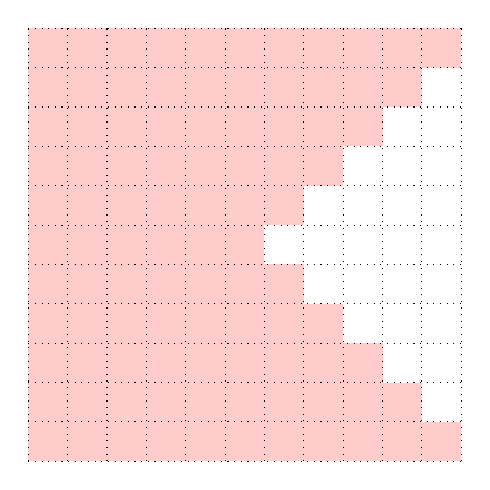
\begin{tikzpicture}
        \fill[fill=red!20](0, 5)--(5.5, 5)--(5.5, 5.5)--(0, 5.5)--cycle;
        \fill[fill=red!20](0, 4.5)--(5, 4.5)--(5, 5)--(0, 5)--cycle;
        \fill[fill=red!20](0, 4)--(4.5, 4)--(4.5, 4.5)--(0, 4.5)--cycle;
        \fill[fill=red!20](0, 3.5)--(4, 3.5)--(4, 4)--(0, 4)--cycle;
        \fill[fill=red!20](0, 3)--(3.5, 3)--(3.5, 3.5)--(0, 3.5)--cycle;

        \fill[fill=red!20](0, 2.5)--(3, 2.5)--(3, 3)--(0, 3)--cycle;%中間
        \fill[fill=red!20](0, 2)--(3.5, 2)--(3.5, 2.5)--(0, 2.5)--cycle;
        \fill[fill=red!20](0, 1.5)--(4, 1.5)--(4, 2)--(0, 2)--cycle;
        \fill[fill=red!20](0, 1)--(4.5, 1)--(4.5, 1.5)--(0, 1.5)--cycle;
        \fill[fill=red!20](0, 0.5)--(5, 0.5)--(5, 1)--(0, 1)--cycle;
        \fill[fill=red!20](0, 0)--(5.5, 0)--(5.5, 0.5)--(0, 0.5)--cycle;
        \draw[dotted, step=0.5cm] (0,0) grid (5.5,5.5);
    \end{tikzpicture}
\end{figure}
ここで,(src.\ref{src:多次元配列の作成})のように,着色部のみの配列を宣言し,そこに文字(列)を代入する工夫をおこなった.
\newpage

\setcounter{section}{2}
\setcounter{subsection}{0}

\section*{課題2}
\noindent\fbox{課題ファイル名}\hspace{1em}\verb|Study01_2.java|
\subsection{大まかな処理過程}
\begin{figure}[h]
    \centering
    \begin{tikzpicture}
        \tikzset{Terminal/.style={rounded rectangle,  draw,  text centered, text width=2cm, minimum height=1cm}};
        \tikzset{Process/.style={rectangle,  draw,  text centered, text width=2cm, minimum height=1cm}};
        \tikzset{Decision/.style={diamond,  draw,  text centered, aspect=3,text width=2cm, minimum height=1cm}};
        \node[Terminal](args)at (-3,0){被検索文字列};
        \node[Process](split)at (-3,-1.5){\verb|split|};
        \node[Process](inArray)at (-3,-3){inArray};
        \node[Process](LookArray)at (-3,-4.5){文字数分配列参照};

        \node[Terminal](input)at (3,0){検索文字列};
        \node[Process](getNumber)at (3,-1.5){文字数取得};
        \node[Decision](Judge)at (0,-6){比較};

        \draw[->,very thick](args)--(split);
        \draw[->,very thick](split)--(inArray);
        \draw[->,very thick](inArray)--(LookArray);
        \draw[->,very thick](LookArray) |- (Judge);

        \draw[->](getNumber) |- (LookArray);
        \draw[->](input)--(getNumber);
        \draw[white,line width=7pt] (input) -| (Judge);
        \draw[->,very thick,](input)-|(Judge);
    \end{tikzpicture}
\end{figure}
\subsection{工夫点}
\noindent\underline{検索メソッドの分離}\par
p.{\pageref{method}}第\ref{method}節でも述べたが,同一の処理をメソッドとしてブロックのように扱うと一連の処理を簡単かつ明瞭にできる.\par
今回は,被検索文字列が,複数あることが前提であり,その被検索文字列を\verb|split|メソッドを用いて分割し,それを配列に代入する.配列に対して行う処理が$1$度ではないので,検索するメソッドを分離することで,処理過程をより見やすくした.\par
\begin{figure}[h]
    \centering
    \begin{tikzpicture}
        \node[rounded corners,fill=cyan!10,rectangle,minimum size=1cm](0){\verb|args[0]|};
        \node[rounded corners,fill=cyan!10,rectangle,minimum size=1cm,right=1cm of 0](1){\verb|args[1]|};
        \node[right=0.5cm of 1](d){\dots};
        \node[rounded corners,fill=cyan!10,rectangle,minimum size=1cm,right=0.5cm of d](n){\verb|args[n]|};
        \node[inner sep=0.3cm,fit={(0)(1)(d)(n)}](wrap_main){};
        \node[inner sep=0cm,above=0.3cm of wrap_main.north west](caption_main){\verb|main|};
        \node[draw,rounded corners,fit={(wrap_main)(caption_main)}](plate_main){};

        \node[diamond,fill=red!10,minimum size=1cm,below=1cm of plate_main](Search){検索};

        \draw[white,line width=4pt,bend right=15]
        (0)     edge (Search)
        (1)     edge (Search)
        (n)     edge (Search);
        \draw[->,bend right=15,dashed]
        (0)     edge (Search)
        (1)     edge (Search)
        (n)     edge (Search);

        \draw[white,line width=4pt,bend right=15]
        (Search)     edge (0)
        (Search)     edge (1)
        (Search)     edge (n);
        \draw[->,bend right=15]
        (Search)     edge (0)
        (Search)     edge (1)
        (Search)     edge (n);
    \end{tikzpicture}
\end{figure}
\centerline{\tikz \draw[dashed,->](0,0)--(1,0)node[right]{配列参照引き渡し};\hspace{1cm}\tikz\draw[->](0,0)--(1,0)node[right]{検索結果(\ttfamily{boolean}\normalfont)値};}
%\newpage
%\noindent\underline{検索を高効率に}

\newpage
\setcounter{section}{3}
\setcounter{subsection}{0}

\section*{課題3}
\noindent\fbox{課題ファイル名}\hspace{1em}\verb|Study01_3.java|
\subsection{大まかな処理過程}
\begin{lstlisting}[caption=ある数に対して素数か否か判定する, label=isPrime, language=Java]
int factorialCounter = 1;// 階乗のカウンタ
for (int i = 2; i <= number; i++) {
    if (number % i == 0) {// numberをiで割った剰余が0ならば,numberはその数を素因数にもつ
        number = number / i;// numberにnumberをiで割った商を代入
        if (number % i == 0) {// もう一度同じ数で割った剰余が0ならば,カウンタをインクリメント
            factorialCounter++;
        } else {
            printPrimeFactor(number, i, factorialCounter);// 素因数を出力するメソッドへ.
            factorialCounter = 1;// カウンタをリセット
        }
        i = 1;
    }
}
\end{lstlisting}
\begin{lstlisting}[caption=その素数が最大であるか判断する, label=maxPrime, language=Java]
public static void printPrimeFactor(int number, int i, int factorialCounter) {
    if (number == 1) {// その素因数が最大の時
        if (factorialCounter == 1) {// その素因数が1乗の時
            System.out.print(i);
        } else {
            System.out.print(i + "^" + factorialCounter);
        }
    } else {// その素因数が最大でない時
        if (factorialCounter == 1) {// その素因数が1乗の時
            System.out.print(i + " * ");
        } else {
            System.out.print(i + "^" + factorialCounter + " * ");
        }
    }
}
\end{lstlisting}
\begin{enumerate}
\renewcommand{\labelenumi}{\arabic{enumi})}
\item 入力数値\verb|number|に対して,ある数\verb|i|で割った剰余が$0$ならば,\verb|number|は\verb|i|を素因数にもつ.
\item 同一の複素数が$2$個以上存在する時,\verb|factoricalCounter|をインクリメントする.(src.\ref{isPrime})
\item 全ての素因数の中で,一番大きいもの以外は,\verb| * |記号を後ろにつけて出力する.(src.\ref{maxPrime})
\item \verb|factoricalCounter|が$2$以上の時,\verb| ^ |記号の後ろに\verb|factoricalCounter|を添える.(src.\ref{maxPrime})
\end{enumerate}
\newpage
\subsection{工夫点}
\noindent\underline{指数カウンタ}\par
はじめ,この問題に取り掛かるとき,配列を用いて解決しようとした.素因数個数分の配列に素因数を昇順に並べる方法である.昇順に並べた素因数が同じもの同士の個数を数えて指数を作る方法をとった.(図\ref{配列を用いた素因数の管理})
しかし,p.\pageref{配列とメモリ}第\ref{配列とメモリ}節にあるように,無駄な変数を置くことは避けた方が良い.\par
\begin{figure}[h]
    \caption{配列を用いた素因数の管理}
    \centering
    \label{配列を用いた素因数の管理}
    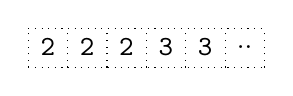
\begin{tikzpicture}
        \tikzset{verb/.style={rectangle,text width=0.25cm,minimum height=0.5cm,text centered}};
        \draw[dotted,step=0.5](0cm,0cm) grid(3cm,0.5cm);
        \node[verb,anchor=south west](0)at(0,0){\verb|2|};
        \node[verb,right=0 of 0]{\verb|2|};
        \node[verb,right=0.5cm of 0]{\verb|2|};
        \node[verb,right=1cm of 0]{\verb|3|};
        \node[verb,right=1.5cm of 0]{\verb|3|};
        \node[verb,right=2cm of 0]{..};
    \end{tikzpicture}
\end{figure}
ここでカウンタを用いると,配列を用いることなく指数の出力が可能になった.(src.\ref{isPrime})
\newpage
\setcounter{section}{4}
\setcounter{subsection}{0}

\section*{課題4}
\noindent\fbox{課題ファイル名}\hspace{1em}\verb|Study01_4.java|
\subsection{大まかな処理過程}
\begin{lstlisting}[caption=コマンドライン引数から曜日シフトを決定, label=曜日シフト, language=Java]
String[] weekName = { "sun", "mon", "tue", "wed", "thu", "fri", "sat" };
String[] week = { "土", "日", "月", "火", "水", "木", "金" };
int weekShift = -1;
for (int i = 0; i < weekName.length; i++) {// コマンドライン引数で曜日シフト数を決定.
    if (args[0].equals(weekName[i])) {
        weekShift = i;
    }
}
\end{lstlisting}
\begin{lstlisting}[caption=経過日数を算出, label=経過日数を算出, language=Java]
int[] daysOfMoth = { 31, 28, 31, 30, 31, 30, 31, 31, 30, 31, 30, 31 };
public static int daysElapsed(int inputMonth, int inputDay, int[] daysOfMoth) {
    int daysElapsed = 0;
    for (int i = 0; i < inputMonth - 1; i++) {
        if (inputMonth == 1) {
            return inputDay;
        }
        daysElapsed += daysOfMoth[i];
    }
    daysElapsed += inputDay;
    return daysElapsed;
}
\end{lstlisting}
\begin{lstlisting}[caption=出力, label=出力, language=Java]
int mod7 = (dayElapsed + weekShift) % 7;
System.out.println(inputMonth + "月" + inputDay + "日は," + week[mod7] +"曜日です.");
\end{lstlisting}
\newpage
\subsection{工夫点}\label{不正検出}
\noindent\underline{ユーザビリティを考慮した設計}\par
コマンドライン入力や日付の入力など,ユーザの動作によって処理する事項は,思わぬエラーを引き起こす.
このプログラムは,あらゆるエラーに対して,エラーメッセージを出力し,プログラムの中止や再入力を促す.\par
エラーメッセージは,基本的に使い回しが多いので,エラーをコード化し,それに対するメッセージを出力するメソッドを作成した.(src.\ref{Eroor})\par
\begin{lstlisting}[caption=エラーメッセージ・メソッド, label=Eroor, language=Java]
public static void printError(int i) {
    if (i == 0)
        System.out.println("調べたい日付が不正な組です");
    else if (i == 1)
        System.out.println("コマンドライン引数の値が不正です");
    else if (i == 2)
        System.out.println("調べたい日付が不正な入力です");
    else if (i == 3)
        System.out.println("演算できませんでした");
}
\end{lstlisting}
コマンドライン引数が不正ではプログラムが動かないので,コマンドライン引数の不正を検出し,\verb|System.exit(0);|で,プログラムを強制終了する.(src.\ref{argsError})
\begin{lstlisting}[caption=コマンドライン引数の不正検出, label=argsError, language=Java]
int weekShift = -1;
if (args.length == 0 || args.length > 1) {// コマンドライン引数が不正の場合(入力なし,または,2つ以上の入力)にエラーを出し,終了
    printError(1);
    System.exit(0);
}

\end{lstlisting}
\newpage
\noindent\underline{日付組み合わせの不正検出}\par
$2$月は$28$日までしかないので,$2$月$30$日と入力があると,エラーである.しかし,全ての月の最後の日付に対して条件分岐を行うと,非常に見難いプログラムになる.そこで,論理演算子と配列を用いて$2$つの条件分岐で日付組み合わせの不正を検出するメソッドを作成した.(src.\ref{日付組み合わせ不正検出})
\begin{lstlisting}[caption=日付組み合わせ不正検出, label=日付組み合わせ不正検出, language=Java]
public static boolean judgeMothAndDate(int inputMonth, int inputDay, int[] daysOfMoth) {// 月日の組み合わせの判定(不正であればFalse)
    if (inputMonth > 12 || inputMonth < 1) {// 不正の条件
        printError(0);
        return false;
    }
    if (1 > inputDay || inputDay > daysOfMoth[inputMonth - 1]) {// 不正の条件
        printError(0);
        return false;
    }
    return true;
}
\end{lstlisting}
これは,\verb|(index + 1)|月の最終日が格納してある配列\verb|dayOfMonth|(src.\ref{経過日数を算出})から不正条件を導き出している.
この検出方法で,この配列と西暦の入力で,閏年の計算も可能になる.\\
\noindent\underline{曜日出力をシンプルに}\par
曜日を出力するために,一般的に\(\textrm{経過日数}\bmod 7\)を計算し,その解に応じて\verb|if|文,\verb|swith|文を使う.$7$の剰余の条件分岐は多行に渡る.非常に見難いプログラムになることは明白である.(src.\ref{switch})\par
ここで,曜日(漢字)を格納する配列を用意し,$7$で割った剰余番目の配列を呼び出すシンプルな仕組みを作成した.(src.\ref{arrayweek})
\begin{lstlisting}[caption=\ttfamily{switch}\normalfont 文を用いたコード例, label=switch, language=Java]
int mod7 = dayElapsed % 7;
switch(mod7){
    case 0:
        System.out.println("土曜日です.");
        break;
    case 1:
        System.out.println("日曜日です.");
        break;
        ・
        ・
        ・
}
\end{lstlisting}
\begin{lstlisting}[caption=配列を用いたコード例, label=arrayweek, language=Java]
String[] week = { "土", "日", "月", "火", "水", "木", "金" };
int mod7 = dayElapsed % 7;
System.out.println( week[mod7] +"曜日です.");
\end{lstlisting}
\newpage
\setcounter{section}{5}
\setcounter{subsection}{0}

\section*{課題5}
\noindent\fbox{課題ファイル名}\hspace{1em}\verb|Study01_5.java|\\
\subsection{大まかな処理過程}
\begin{lstlisting}[caption=コマンドライン引数の不正を検出, label=argsE, language=Java]
if (args.length != 2) {
    System.out.println("コマンドライン引数は2つです");
    System.exit(0);
}
int firstNumber = Integer.parseInt(args[0]);
int secondNumber = Integer.parseInt(args[1]);
int linesCounter = 0;
if (firstNumber > 1000 || firstNumber < 1 || secondNumber > 1000 || secondNumber < 1) {
    System.out.println("コマンドライン引数は1以上1000以下を入力してください");
    System.exit(0);
}
\end{lstlisting}
\begin{lstlisting}[caption=コマンドライン引数の大小比較・条件分岐, label=大小比較, language=Java]
if (firstNumber < secondNumber) {// 昇順
    for (int i = firstNumber; i <= secondNumber; i++) {
        if (isPrime(i) == true) {
            System.out.printf("%4d", i);
            if (linesCounter == 11) {// 改行判断
                System.out.println();
                linesCounter = 0;
            } else {
                linesCounter++;
            }
        }

    }
} else {...
\end{lstlisting}
\begin{lstlisting}[caption=素数判断, label=isPPrime, language=Java]
public static boolean isPrime(int i) {// 素数であればTrue
    if (i == 1) return false;
    if (i % 2 == 0 && i != 2) return false;
    double sqrtI = Math.sqrt(i);
    for (int j = 3; j <= sqrtI; j += 2) {
        if (i % j == 0) return false;
    }
    return true;
}
\end{lstlisting}
\subsection{工夫点}
\noindent\underline{コマンドライン引数での不正を検出}\par
p.\pageref{不正検出}第\ref{不正検出}章と同じく,コマンドライン引数でエラーを検出し,プログラムを終了する仕組みを作成した.(src.\ref{argsE})\\
\noindent\underline{出力終了ラインの調整}\par
この問題は$12$列の素数出力で改行する必要がある.細かいところだが,ちょうど$12$列の出力の場合,最終出力行の次の行に\verb| = |で造られた出力終了ラインを出力する必要がある.そのことを考慮した結果と,考慮しなかったっ結果を比べる.
当然だが,考慮した方が題意に沿っている.
\begin{itembox}[l]{考慮しなかった場合}
        \verb|$ java Study01_5 3 41| \ovalbox{Enter}\\
        \verb|=============   3から  41までの素数=============|\\
        \verb|   3   5   7  11  13  17  19  23  29  31  37  41|\\\\
        \verb|================================================|
\end{itembox}
\begin{itembox}[l]{考慮した場合}
    \verb|$ java Study01_5 3 41| \ovalbox{Enter}\\
    \verb|=============   3から  41までの素数=============|\\
    \verb|   3   5   7  11  13  17  19  23  29  31  37  41|\\
    \verb|================================================|
\end{itembox}
列数カウンタ(\verb|linesCounter|)に対して,条件分岐を設けた.(src.\ref{linesCounter})
\begin{lstlisting}[caption=列数カウンタによる条件分岐, label=linesCounter, language=Java]
if (linesCounter == 0) {// 最後の数値が12列目か否か
    System.out.println("================================================");
} else {
    System.out.println();
    System.out.println("================================================");
}
\end{lstlisting}

\noindent\underline{素数判断の効率化}\par
素数判定について,「素数でない数$x$は$\sqrt{x}$以下の約数をもつ」という性質を用いれば,劇的に処理が速くなる.(src.\ref{isPPrime})\par
本来(src.\ref{isPrimeb}),ある数\verb|i|に対して,その数が$2$以上,\verb|i|以下で割り切れるかどうかを判定するが,src.\ref{isPPrime}では,その数の$1/2$乗の数までのみ剰余演算をし,ループ回数が大幅に減って処理速度が大きくなる.
\begin{lstlisting}[caption=素数判定の基本, label=isPrimeb, language=Java]
    if (i == 1) return false;
    if (i == 2) return true;
    for (int j = 2; j < i; j++) {
        if (i % j == 0) return false;
    }
    return true;
\end{lstlisting}
\end{document}